\section{Terms of Definition}
\label{sec:terms_of_definition}
In this section the term \textit{intimate} is defined. Due to this it is considered which data is perceived as intimate and in which circumstances.
Answering the first research question in this work is not as easy as it seems. Therefore, several definitions from different source are collected.

The perceiving of what is intimate depends on several factors.
In general it has to be differentiate between the culture, how a human is perceiving the self and which factors are shaping the sociocultural live \cite{carrithers1985category}. It is not possible to consider all well-known cultures in this work, therefore the focus is limited to the scrutiny of the western civilization. 
\begin{figure}[htb]
	\centering
	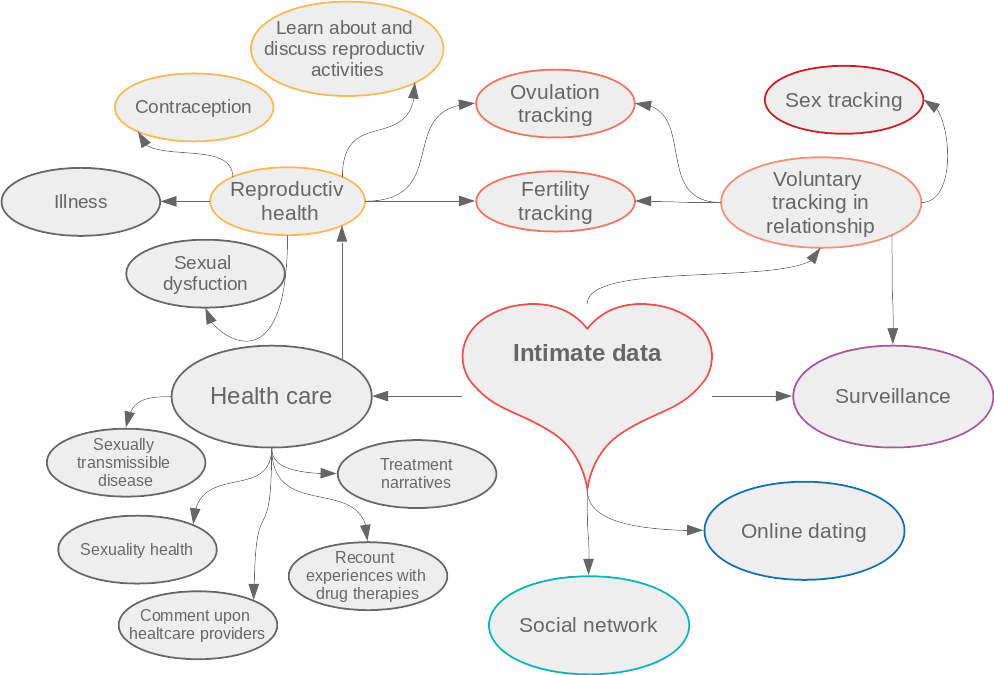
\includegraphics[width=\linewidth]{img/cluster_heart.png}
	\caption{Visualization of possible intimate data, which are arising from using such digital technologies.}
	\label{fig:cluster}
\end{figure}
In the western civilization or rather in the \ac{EU} privacy and data security takes up more attention, even since the \ac{GDPR} is applied \cite{albrecht2016gdpr}.
However, the state of a person in the society is defining the personal perception of privacy and data security, and the personal view as well. What is perceived as intimate depends on this factors.
But these can not be defined in a few sentences, the topic is to complex and not measurable. Furthermore, it is subjective. For the individual, the perception of whether data are intimate or not is different. 
Several works are focused on intimate data in different contexts. Although, which data is intimate or what people perceive as intimate is not clearly defined. Due to this, some descriptions are summarized to give a rough outline.

The focus in Danaher et al. \cite{doi:10.1080/15265161.2017.1409823} is on intimate interpersonal relationships. In this work no clear definition of the term intimate data is presented. They argued that it does not need a precise definition to get an understanding of intimate relationships. To describing a romantic relationship the authors wrote:

\begin{quote}
	[...] we trust that most readers' intuitive sense of those terms [..] will be adequate for our arguments to make sense. That said, "romantic relationship" might usefully be thought of as a cluster concept, with paradigmatic examples in the middle, and less paradigmatic examples clustered around it, each one different along various dimensions (e.g., the degree to which sexual interaction is central to the relationship).
\end{quote}

If it is possible to define an intimate or romantic relationship about such a way, this concept will also work for the term intimate. 
The term \textit{intimate} can be visualized in a cluster of different types of intimate data, which are assigned to corresponding activities, e.g. fertility tracking.
In figure \ref{fig:cluster} several topics related to the term intimate data are collected and brought in relation to each other. At this point it must be emphasized that this does not cover the complete field, in which intimate data would be collected, tracked, shared and so on. Rather it is an summarization of terms and descriptions which come up in this work.

%from Levy \cite{levy2014intimate}, Danaher et al. \cite{doi:10.1080/15265161.2017.1409823}, Lupton \cite{doi:10.1080/13691058.2014.920528} and more. 

The idea to use an cluster concept can be thought of one step further. The sensitivity or level of intimate data could be arranged in some sort of data hierarchy. Form IT-Security Management it is known to evaluate risks by assigning a probability and to classify accordingly (see documentation of Federal Office for Information Security (BSI) \cite{bsi}). In this table I want to classify the data summarized above based on their sensibility.
%TODO: Tabelle über die oben genannten Daten einfügen mit Einstufung; Stufung bestimmen

To give another understanding of what is meant with \textit{intimate} in this paper I want to quote a paragraph form Lupton \cite{doi:10.1080/13691058.2014.920528}, which describes an Application for mobile phones:
\begin{quote}
	The	Glow app brings male partners into the equation by sending them a digital
	message when their partner is in her fertile period and reminding them to bring her flowers	[...]. This app also tracks menstrual and ovulation indicators, as well as asking women to enter details of their sexual encounters, including sexual positions used, whether or not they had an orgasm and whether they experienced emotional or physical discomfort during sex. It employs the aggregated data from other users to refine predictions of ovulation and fertility for the individual user. [...]
\end{quote}
This paragraph describes a sort of tracking which also called \textit{intimate tracking} (defined by \cite{doi:10.1080/15265161.2017.1409823}).

We can also find intimate data also in other contexts, e.g. as mentioned above in health care.
%TODO: finde Quellen zu Aufsätzen intimer Daten in Verbindung mit Drogensucht
But the focus in this paper is on intimate data in relationships, therefore it is referred to the figure \ref{fig:cluster} above. This should give a general understanding of the context. 
